\chapter{Deep Learning method for Changes Detection}
The previous approach, called the classical approach, has a big drawback. For each new shape targeted for change detection, such as spheres, and cylinders, it necessitates a specific implementation, resulting in the need for adaptation of the entire pipeline.\\

Recent progress in deep learning methods has shown promising results in the classification and semantic segmentation of complex objects or scenes \cite{DeepLearningPointCloud}. Consequently, this second approach investigates the potential of a neural network to tackle the previous limitation, allowing the detection of changes in complex shapes thereby providing a realistic framework for real-world scenarios.\\

In this chapter, we first introduce key concepts of neural networks. It is followed by a review of three networks, namely PointNet, PointNet++, and FlowNet3D, which are relevant to this master thesis. Finally, we propose a network tailored for the change detection purpose.

\section{Fundamentals of Neural Networks}
This section provides a comprehensive overview of the fundamental concepts of neural networks and their training process \cite{LINFO2262}. 
\subsection{Overview of Artificial Neural Networks}
Artificial Neural Networks (ANNs) are computational models inspired by the structure and function of biological brains. They consist of interconnected nodes, called neurons or units, organized into layers. Each neuron receives inputs, processes them, and produces an output signal.\\

Neurons are the basic building blocks of neural networks. Each neuron applies a mathematical operation to its inputs, typically a weighted sum followed by an activation function. The activation function introduces non-linearities and allows neural networks to model complex relationships in the data.
\begin{figure}[H]
    \begin{minipage}{0.5\textwidth}
        \centering
        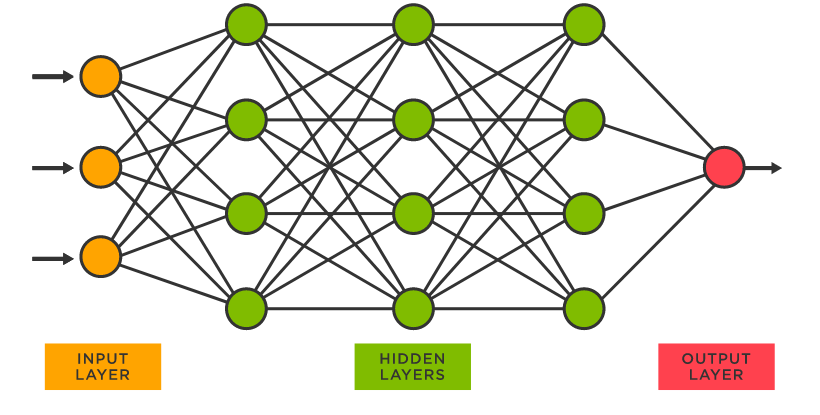
\includegraphics[width=\textwidth]{Img/05_ANN.png}
        \caption{ANNs basic architecture \cite{ANN}}
        \label{fig:ANNs}
    \end{minipage}
    \begin{minipage}{0.5\textwidth}
        \centering
        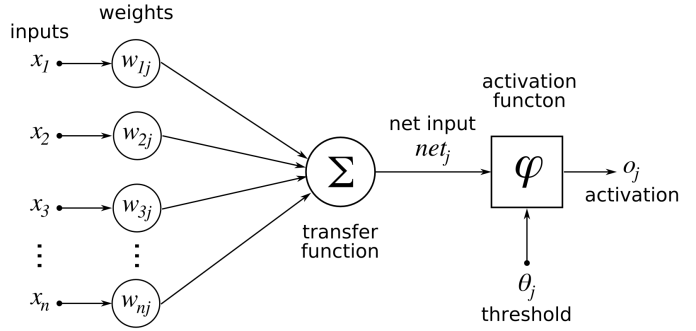
\includegraphics[width=\textwidth]{Img/05_Neuron.png}
        \caption{Interaction for a single neuron \cite{neuron}}
        \label{fig:Neuron}
    \end{minipage}
\end{figure}

\subsection{Feedforward and Backpropagation}
Feedforward is the process of passing data through a neural network from the input layer to the output layer. During feedforward, each neuron's output becomes the input for the neurons in the subsequent layer. Backpropagation is the algorithm used to train neural networks by adjusting the weights based on the difference between the predicted output and the ground truth.

\subsection{Training and Optimization}
Training a neural network involves optimizing its weights to minimize a defined loss function. This is done through an optimization algorithm, such as gradient descent, which iteratively adjusts the weights based on the computed gradients. The learning rate and the choice of optimization algorithm play crucial roles in training efficiency and convergence.


\subsection{Loss Functions}
Loss functions quantify the discrepancy between the predicted outputs and the ground truth labels. Different tasks and applications require specific loss functions, such as mean squared error for regression problems or cross-entropy loss for classification tasks.

\section{PointNet}
PointNet is a deep learning architecture designed to process point clouds. It can be supplemented with attributes such as colors, intensity, or normals. It is one of the pioneering architectures that achieves good results on many classification tasks and semantic segmentation tasks \cite{PointNet}.\\

The authors of PointNet identified three key challenges in processing point clouds:
\begin{itemize}
    \item First, point clouds lack a specific structure and are unordered, unlike grids or meshes.
    \item Secondly, each data point interacts directly with its local neighbors forming structures. This interaction becomes particularly significant in segmentation tasks, where local structures may correspond to different classes.
    \item Finally, the point cloud should be invariant under permutation and transformation. This signifies that two point clouds can represent the same object, although the points are described in a different order. Additionally, invariance under transformation means rotation or translation of a whole point cloud can represent the same properties.
\end{itemize}

\subsection{PointNet architecture}
\begin{figure}[ht]
    \centering
    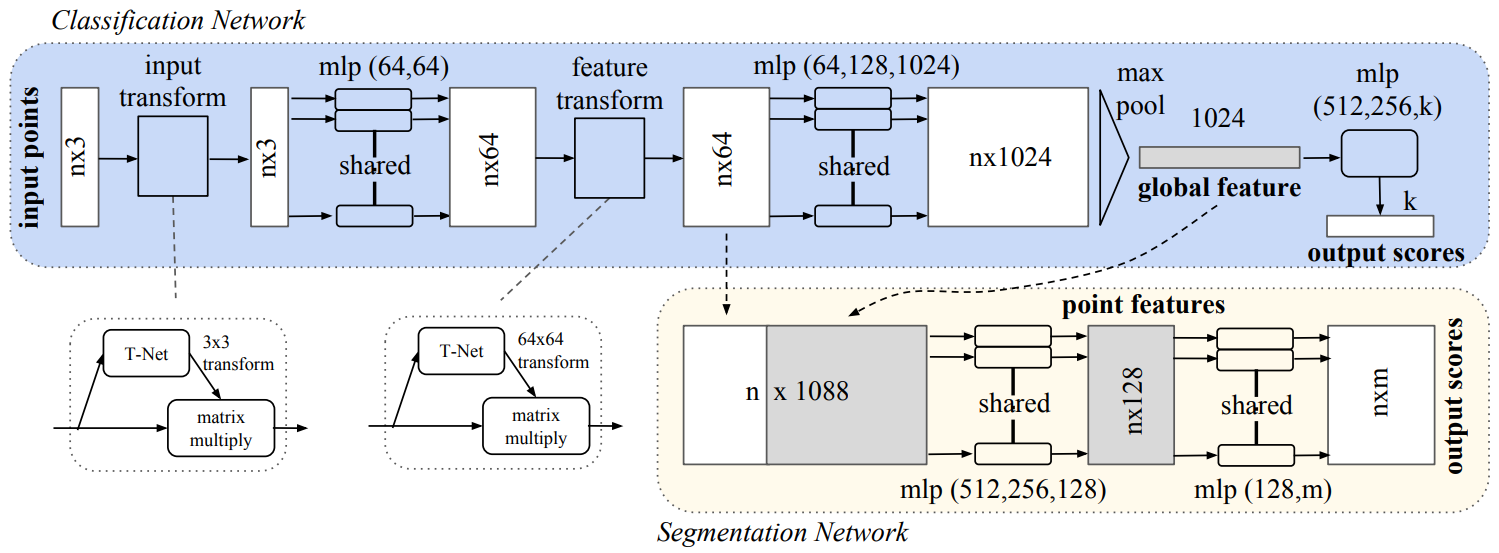
\includegraphics[width=\textwidth]{Img/05_Pointnet.png}
    \caption{PointNet Architecture \cite{PointNet}}
    \label{fig:Pointnet1}
\end{figure}
PointNet offers a solution that tackles the previously mentioned challenges. The architecture of PointNet, illustrated in Figure \ref{fig:Pointnet1}, can be separated into two networks: the classification and segmentation one. As their name suggests, each network has different objectives and outputs. \\
\subsubsection{Classification}

As shown in Fig \ref{fig:Pointnet1}, the classification network undergoes an 'input transform', followed by a shared multi-layer perceptron (MLP) and a 'feature transform'. Once those steps are done, the network obtains $n\times 64$ local features .\\

The 'input transform' and 'feature transform' are essential to the network as they predict a transform that projects input points (in the input transform) or input features (in the feature transform) in a canonical space ensuring points and features invariance under transformation which is one of the challenges of points data mentioned earlier. Those essential transformations have recourse to the \textbf{Joint Alignment Network}, which utilizes a network called T-Net that predicts the transformation matrix to achieve invariance.\\

For classification, the main interest is the global features of the point cloud, enabling discrimination between different classes. To achieve this, local features enter a shared MLP followed by a \textbf{max pooling} layer. This max pooling layer is also critical for the network. Selecting the maximum value for each feature ensures invariant global features of the point cloud. \\

Once the global feature vectors are obtained, it goes through a fully connected MLP layer to obtain an output classification score. The predicted class is simply the one where the score is maximum. 

\subsubsection{Segmentation}
The segmentation network can be viewed as an extension built upon the preceding classification network. It concatenates global and local features to generate points features, which will be processed through a MLP, to produce per-point output scores. By utilizing both local and global features, it achieves scene understanding, capturing local and global interaction between points.

\subsection{Why PointNet}
Our main motivation for utilizing PointNet, and its improvement PointNet++, stems from their pioneering ability to directly process point clouds. PointNet has shown good results on different benchmarks. For example, in classification task, the method reached an accuracy of $89.2\%$ on the ModelNet40 dataset, which encompass synthetic object split into 40 categories \cite{modelnet}. For semantic classification, it performed with a mean accuracy of $78.9 \%$ on S3DIS, an indoor scene dataset consisting mostly of rooms and hallways relevant for our purpose \cite{s3dis}.\\

Moreover, its value lies in its ability to directly learn from raw point cloud data, eliminating the requirement for manual feature engineering or complex preprocessing steps. This aspect becomes especially advantageous when compared to other networks, such as RandLA-Net, that typically rely on additional structured inputs or handcrafted features derived from complex preprocessing pipelines \cite{Randla-net}.\\

Considering the satisfactory results, the availability of implementations, and the user-friendly nature of the network, we decided to investigate PointNet for our research.

\section{PointNet++}
PointNet++, sometimes denoted as PointNet 2, is built upon the original PointNet architecture by addressing some of its limitations and improving its performance. The main enhancement introduced by PointNet++ is the ability to capture local features from the point cloud data in a structured and hierarchical manner \cite{PointNet2}.\\

Instead of processing each point independently, PointNet++ introduces a hierarchical neural network architecture that takes into account the local structures and relationships between points. It achieves this by dividing the input point cloud into a series of nested partitions called "local regions."

\subsection{PointNet++ architecture}
\begin{figure}[ht]
    \centering
    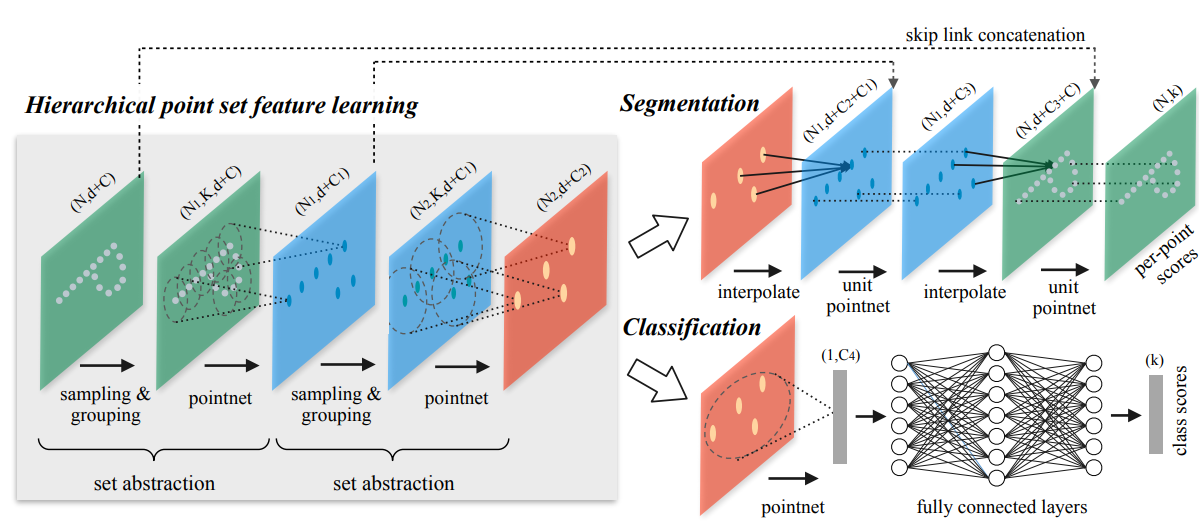
\includegraphics[width=\textwidth]{Img/05_Pointnet2.png}
    \caption{PointNet++ architecture \cite{PointNet2}.}
    \label{fig:Pointnet2}
\end{figure}

The PointNet++ architecture is characterized by a hierarchical structure comprising several stages referred to as set abstraction levels. Each set abstraction level encompasses three key layers: a 'sampling layer', a 'grouping layer', and a 'PointNet layer'.\\

In the sampling layer $l$, the purpose consists in selecting a predetermined number of points $N_l$ from the input data. The selection of these points is not random. Instead, a technique called \textbf{farthest point sampling} selects points. This technique ensures the $N_l$ chosen points evenly cover the input data and thus, captures its essential structure while reducing the computational complexity.\\

Following the sampling layer, the grouping layer search for local points surrounding the selected $N_l$ centroids. It is achieved through a method called \textbf{ball query} which associates each centroid with its neighboring points within a specified radius.\\

Within each local region, PointNet++ applies the same set of operations as PointNet to extract $C$ global features for each $N_l$ point. The output of the set abstraction layer consists of $N_l$ points, each represented by a vector of size $d+F$ where $d$ represents the input dimension, typically of size 3 or 6, and $F$ is the number of global features.\\

By applying iteratively the set abstraction layer, PointNet++ captures a hierarchy of features in a more structured manner. At each subsequent level, the considered regions become more global and capture increasingly global details. The final output of the multiple levels is a collection of hierarchical features that encompass both local and global information for a subsampled input point cloud.\\

\subsubsection{Classification}
Regarding classification tasks, the output after applying different set abstraction layers is a set of shape $(N_l,d+C)$ capturing both local and global features. On this set, a PoinNet layer for classification can be applied just as in Figure \ref{fig:Pointnet1}.

\subsubsection{Semantic segmentation and Point Feature Propagation}
When it comes to semantic segmentation tasks, directly applying PointNet to the output of the set abstraction layers is not suitable. This is because the $N_l$ points obtained from the layers represent a subsampling of the input point set and it requires an additional upsampling step.\\

To tackle this challenge, PointNet++ adopts a hierarchical propagation strategy utilizing distance-based interpolation and skip links across different levels. At each feature propagation level, the point features of size $(N_{l},d + F) $ are propagated to $N_{l-1}$ points, where $N_{l-1}$ and $N_{l}$ denote the point set sizes of the input and output of the set abstraction level $l$ ($N_{l-1} \geq N_l$) respectively.\\

Feature propagation is achieved by interpolating the feature values of $N_{l}$ points at the coordinates of the $N_{l-1}$ points. Inverse distance weighted average interpolation, based on the $k$ nearest neighbors, is utilized as shown in Equation \ref{InvDist}. The interpolated features on the $N_{l-1}$ points are then concatenated with the previous point features obtained from the set abstraction level $l-1$.
\begin{equation}\label{InvDist}
f^{(j)}(x)=\frac{\sum_{i=1}^k w_i(x) f_i^{(j)}}{\sum_{i=1}^k w_i(x)} \quad \text { where } \quad w_i(x)=\frac{1}{d\left(x, x_i\right)^2}, j=1, \ldots, F
\end{equation}
The concatenated features are passed through a 'unit PointNet', which is equivalent to the PointNet segmentation network illustrated in Fig \ref{fig:Pointnet1}.\\

This process is repeated until the features are propagated to the original set of points, ensuring that the per-point scores and labels are obtained for the entire point cloud.

\section{FlowNet3D}
Flownet3D is a deep learning architecture designed specifically for point cloud data, enabling the estimation of 3D motion between two point clouds. It builds upon the concept of optical flow, which is a technique used in computer vision to estimate the motion of pixels between consecutive frames in a video sequence \cite{FlowNet}.
\begin{figure}[H]
    \centering
    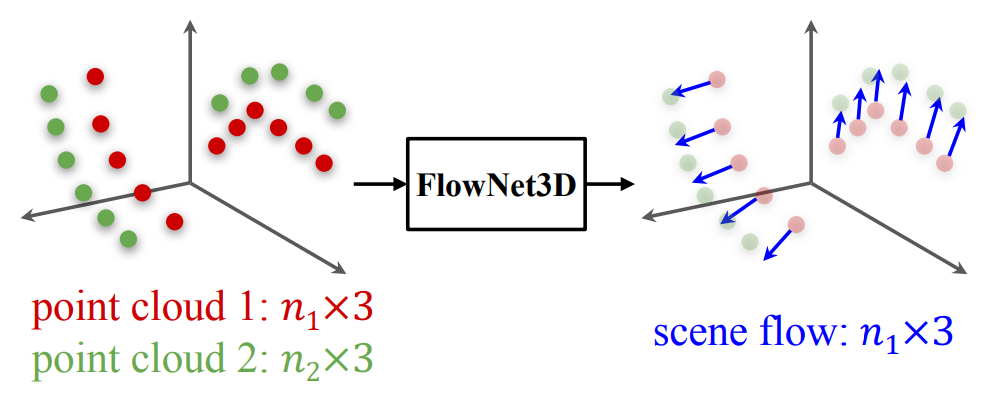
\includegraphics[width=\textwidth]{Img/05_Flow3D.png}
    \caption{Scene flow estimation from point clouds \cite{FlowNet}}
    \label{fig:flow}
\end{figure}
The goal of FlowNet3D is to estimate the correspondences between points in two input point clouds and infer the 3D motion vector for each point. This information can be useful for various applications, such as motion tracking, scene reconstruction, and understanding the dynamics of 3D objects or scenes.

\subsection{FlowNet3D architecture}
\begin{figure}[H]
    \centering
    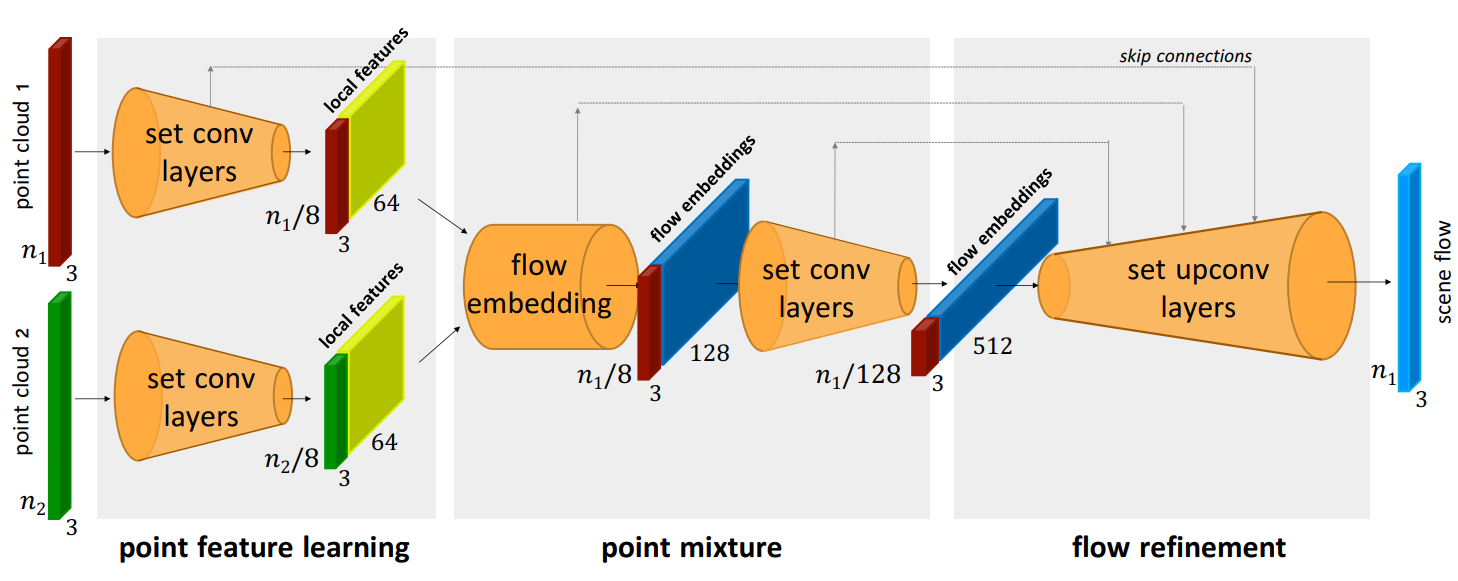
\includegraphics[width=\textwidth]{Img/05_FlowNet3D.png}
    \caption{FlowNet3D Architecture \cite{FlowNet}.}
    \label{fig:FlowNet}
\end{figure}
The network consists of three key modules: 'point feature learning', 'point mixture', and 'flow refinement'. Each module is supported by specific layers, including 'set conv layers', 'flow embedding layers', and 'set upconv layers'.\\

The point feature learning is done by a set conv layer. This layer is based on the PointNet++ set abstraction layer architecture. It takes as input a point cloud and outputs a sub-sampled point cloud with hierarchical features. As previously explained, this layer uses the farthest point sampling and ball query method to select representatives to extract local features which capture spatial locality and translation invariance.\\

The point mixture module uses a flow embedding layer to mix two point clouds and a set conv layer. Flow embedding aggregates flow votes from neighboring points in the second frame to estimate point motions. It considers both geometric feature similarities and spatial relationships to encode point motions. It employs a non-linear function and element-wise max pooling to compute flow embeddings.\\

The flow refinement module involves the set upconv layer, which up-samples the final flow embedding obtained. The set upconv layer aggregates neighboring source points' features using a similar strategy as the set conv layer but with a different local region sampling approach. Similarly to PointNet++ in Fig \ref{fig:Pointnet2}, the network includes skip connections that concatenate set conv output features to facilitate information flow.

\subsection{Why FlowNet3D}

Estimation of 3D motion between two point clouds is relevant in the context of change detection between point clouds. These motion flows represent desirable features that can be leveraged for classifying or segmenting various changes. FlowNet3D is a network specifically designed for this purpose.\\

Furthermore, it is noteworthy that the authors of FlowNet3D are also involved in the development of PointNet and PointNet++, revealing coherence and consistency among these networks.\\

Additionally, different implementations with pre-trained models are available which allows us to rapidly evaluate the proof of concept in this master thesis. These factors, collectively combined, contribute significantly to the decision of selecting this network.\\

However, it is important to acknowledge that there exists a set of less established methods that demonstrated superior performance over FlowNet3D \cite{Flow3D}

\section{Proposed Network}
The goal of our network is to either classify or segment construction faults within an input point cloud based on a reference point cloud representing the same scene. For that purpose, we developed a network designed to detect faults in a manner that is transferable and easily adaptable when new types of faults are introduced.
\begin{figure}[H]
    \centering
    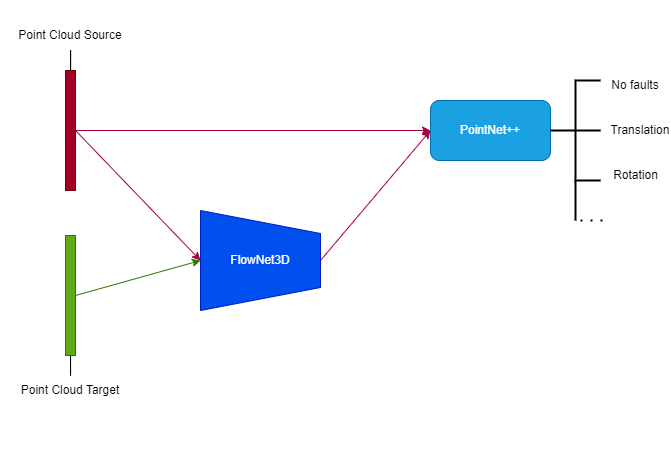
\includegraphics[width=\textwidth]{Img/05_OurNetwork.png}
    \caption{Our construction fault classifier/segmentation network}
    \label{fig:Ours}
\end{figure}
The proposed network architecture comprise two main components: FlowNet3D and PointNet++. It takes a pair of input point clouds, representing different frames of the same scene, and produces a semantic segmentation or classification of potential changes that have occurred.\\

First, FlowNet3D is applied to the pair of point clouds. FlowNet3D estimates the scene flow, which captures the points' motion between those two frames by leveraging the spatial information in both point clouds. The displacement vectors provide temporal information about the motion between the frames.\\

Next, the estimated scene flow is then combined with the source point cloud and fed into PointNet++. This integration allows the network to take into account spatial and temporal information, crucial for change detection.\\

Finally, PointNet++ produces the desired output based on the specific task at hand, whether it is a classification or a semantic segmentation. 